\documentclass[10pt,x11names,table]{beamer}

\usetheme[progressbar=frametitle]{metropolis}
\usepackage{appendixnumberbeamer}
\usepackage{xcolor}

\usepackage{polyglossia}
\setmainlanguage{spanish}

\usepackage{listings}

\usepackage{booktabs}
\usepackage[scale=2]{ccicons}

\usepackage{pgfplots}
\usepgfplotslibrary{dateplot}

%ANIMACIONES
\usepackage{animate}
\usepackage{graphicx}
\usepackage[caption=false]{subfig}

\usepackage{xspace}

\newcommand*{\eg}{e.g.\@\xspace}
\newcommand*{\ie}{i.e.\@\xspace}

\let\oldquote\quote
\let\endoldquote\endquote
\renewenvironment{quote}[2][]
  {\if\relax\detokenize{#1}\relax
     \def\quoteauthor{#2}%
   \else
     \def\quoteauthor{#2~---~#1}%
   \fi
   \oldquote}
  {\par\nobreak\smallskip\hfill(\quoteauthor)%
   \endoldquote\addvspace{\bigskipamount}}
   
\usepackage{wrapfig}

\usepackage{subfig}
\usepackage{hyperref}
\usepackage{multicol}

\setbeamertemplate{bibliography item}[text]

\usepackage[font=small,skip=0pt, labelformat=empty]{caption}

\usepackage{dirtytalk}
\usepackage[acronym]{glossaries}
\makeglossaries

\newacronym{acgan}{ACGAN}{Auxiliary Classifier GAN}
\newacronym{ae}{AE}{Autoencoder}
\newacronym{ai}{AI}{Artificial Intelligence}
\newacronym{api}{API}{Application Programming Interface}
\newacronym{bert}{BERT}{Bidirectional Encoder Representations from Transformers}
\newacronym{brief}{BRIEF}{Binary Robust Independent Elementary Features}
\newacronym{brnn}{BRNN}{Bidirectional RNN}
\newacronym{bptt}{BPTT}{Backpropagation Through Time}
\newacronym{cbow}{CBOW}{Continous bag-of-words}
\newacronym{cnn}{CNN}{Convolutional Neural Network}
\newacronym{crnn}{CRNN}{Convolutional Recurrent Neural Network}
\newacronym{ddpm}{DDPM}{Denoising Diffusion Probabilistic Model}
\newacronym{ddim}{DDIM}{Denoising Diffusion Implicit Model}
\newacronym{diffit}{DiffiT}{Diffusion Vision Transformer}
\newacronym{dl}{DL}{Deep Learning}
\newacronym{dnn}{DNN}{Deep Neural Network}
\newacronym{dos}{DoS}{Denial of Service}
\newacronym{drnn}{DRNN}{Deep Recurrent Neural Network}
\newacronym{ecg}{ECG}{Electrocardiogram}
\newacronym{elmo}{ELMo}{Embedding from Language Model}
\newacronym{fast}{FAST}{Features from Accelerated Segment Test}
\newacronym{fid}{FID}{Fréchet Inception Distance}
\newacronym{foss}{FOSS}{Free and open-source software}
\newacronym{gan}{GAN}{Generative Adversarial Network}
\newacronym{glove}{GloVe}{Global Vectors for Word Representation}
\newacronym{gpu}{GPU}{Graphics Processing Unit}
\newacronym{gru}{GRU}{Gated Recurrent Unit}
\newacronym{ilsvrc}{ILSVRC}{ImageNet Large Scale Visual Recognition Challenge}
\newacronym{is}{IS}{Inception Score}
\newacronym{kid}{KID}{Kernel Inception Distance}
\newacronym{ldm}{LDM}{Latent Diffusion Model}
\newacronym{lstm}{LSTM}{Long Short-Term Memory}
\newacronym{mape}{MAPE}{Mean Absolute Perentage Error}
\newacronym{ml}{ML}{Machine Learning}
\newacronym{mlp}{MLP}{Multilayer Perceptron}
\newacronym{mmd}{MMD}{Maximum Mean Discrepancy}
\newacronym{mse}{MSE}{Mean Squared Error}
\newacronym{ner}{NER}{Named Entity Recognition}
\newacronym{nlg}{NLG}{Natural Language Generation}
\newacronym{nlp}{NLP}{Natural Language Processing}
\newacronym{nlu}{NLU}{Natural Language Understanding}
\newacronym{nn}{NN}{Neural Network}
\newacronym{ocr}{OCR}{Optical Character Recognition}
\newacronym{onnx}{ONNX}{Open Neural Network Exchange}
\newacronym{pmml}{PMML}{Predictive Model Markup Language}
\newacronym{relu}{ReLU}{Rectified Linear Unit}
\newacronym{rest}{REST}{Representational State Transfer}
\newacronym{rnn}{RNN}{Recurrent Neural Network}
\newacronym{sae}{SAE}{Stacked Autoencoder}
\newacronym{sift}{SIFT}{Scale-Invariant Feature Transform}
\newacronym{slam}{SLAM}{Simultaneous Localization and Mapping}
\newacronym{sru}{SRU}{Single Recurrent Unit}
\newacronym{surf}{SURF}{Speeded-Up Robust Features}
\newacronym{svm}{SVM}{Support Vector Machine}
\newacronym{vae}{VAE}{Variational Autoencoder}
\newacronym{vgg}{VGG}{Visual Geometry Group}
\newacronym{vit}{ViT}{Vision Transformer}
\newacronym{wsgi}{WSGI}{Web Server Gateway Interface}
\newacronym{xai}{XAI}{eXplainable Artificial Intelligence}
\newacronym{yolo}{YOLO}{You Only Look Once}
\newacronym{zsl}{ZSL}{Zero-shot Learning}
\subtitle{Métodos Generativos, curso 2024-2025}

\date{\today}
\author{Guillermo Iglesias, guillermo.iglesias@upm.es \newline
Jorge Dueñas Lerín, jorge.duenas.lerin@upm.es  \newline
Félix Fuentes Hurtado, felix.fuentes@upm.es}

\institute{Escuela Técnica Superior de Ingeniería de Sistemas Informáticos | UPM \newline
\hbox{} \newline \ccbysa \hspace{0.1pt} \ccNonCommercial}

%%%%%%%%%%%%%%%%%%%%%%%%%%%%%%%%%%%%%       
\title{Data augmentation para imágenes}

\begin{document}
\maketitle

\section{Introducción al Data Augmentation}

\begin{frame}{Motivación}
Cuando se realiza un \alert{entrenamiento} con redes neuronales uno de los aspectos que más \alert{limitan su rendimiento} es la falta de datos.

Cabe recordar que las redes neuronales son modelos \alert{altamente exigentes} con la disponibilidad de datos. La \alert{convergencia}, \alert{rendimiento}, \alert{resistencia al overfitting} o \alert{estabilidad} son algunos de los aspectos sensibles a la variabilidad en los datos.

\begin{figure}
    \centering
    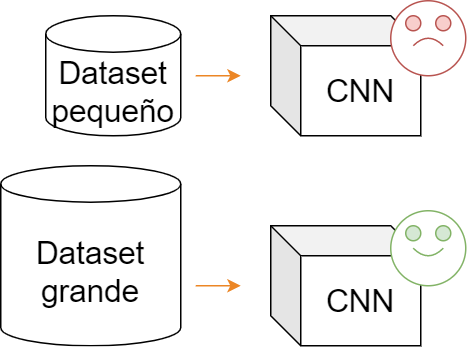
\includegraphics[width=0.6\textwidth]{Slides/figures/Tema 3/DA_Performance.png}
\end{figure}
\end{frame}

\begin{frame}{¿Qué es el data augmentation?}
El proceso de \alert{data augmentation} tiene como objetivo \alert{aumentar sintéticamente} el tamaño del dataset que se usa. Para ello se aplican diferentes \alert{transformaciones} al conjunto de datos que se tiene.

Con ello se obtienen \alert{más datos} a partir de la información que se tiene originalmente. La \alert{calidad} de estos datos dependerá de los algoritmos utilizados, el objetivo que se busca es \alert{replicar} lo más fielmente la distribución de datos original.

\begin{figure}
    \centering
    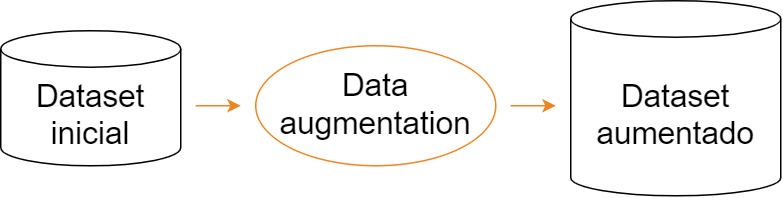
\includegraphics[width=\textwidth]{Slides/figures/Tema 3/DA_Scheme.png}
\end{figure}
\end{frame}

\begin{frame}{Data augmentation como replica de la distribución de datos}
Desde un punto de vista matemático, se pretender \alert{replicar la distribución} de datos original, con cierta \alert{variabilidad} en los nuevos datos, pero manteniendo su \alert{distribución original}. Se busca generar nuevas instancias \alert{indistinguibles} de las originales.

\begin{figure}
    \centering
    \includegraphics[width=0.4\textwidth]{Slides/figures/Tema 3/Distribución 1.png}
\end{figure}
\end{frame}

\begin{frame}{Data augmentation como replica de la distribución de datos}
Desde un punto de vista matemático, se pretender \alert{replicar la distribución} de datos original, con cierta \alert{variabilidad} en los nuevos datos, pero manteniendo su \alert{distribución original}. Se busca generar nuevas instancias \alert{indistinguibles} de las originales.

\begin{figure}
    \centering
    \includegraphics[width=0.4\textwidth]{Slides/figures/Tema 3/Distribución 2.png}
\end{figure}
\end{frame}

\begin{frame}{Ventajas de uso de data augmentation}
En el campo de las \alert{redes neuronales artificiales} el uso de técnicas de aumento de datos permite \alert{mejorar el rendimiento} en ciertos aspectos:
\begin{itemize}
    \item \alert{Overfitting}: Una de las principales causas de este problema es que los modelos son capaces de \say{\alert{aprender}} los casos con los que fueron entrenados.
    \item \alert{Mejor rendimiento}: Al conseguir una distribución de datos más rica se consiguen mejores \alert{precisiones} a la hora de clasificar, al permitir a la red una mejor \alert{generalización}.
\end{itemize}
\end{frame}

\begin{frame}{Implementaciones del data augmentation}
Las técnicas de data augmentation, se utilizan para \alert{todo tipo de datos}, independientemente de su origen. Sin embargo, \alert{no todas las técnicas} pueden ser aplicadas a \alert{todos los conjuntos} de datos de la misma manera.

Existen algoritmos de \alert{data augmentation} específicos para distintos tipos de datos:
\begin{itemize}
    \item \alert{Señales}
    \item \alert{Imágenes}
    \item \alert{Datos tabulares}
\end{itemize}

Como norma general, las técnicas aplicadas deben ser cuidadosamente \alert{estudiadas} para adaptarse al \alert{problema} que se trate concreto.
\end{frame}

\section{Data augmentation para imágenes}

\begin{frame}{Introducción}
Existen un conjunto de técnicas de data augmentation que se pueden aplicar de manera general a las \alert{imágenes}. Una de las ventajas de las imágenes es su \alert{fácil comprensión} debido a que los resultados pueden ser \alert{validados de manera visual}.

Sin embargo, cada \alert{problema es distinto} y no siempre será posible aplicar todas las técnicas a cualquier problema. Siempre debe ser analizado \alert{cómo modifican} los algoritmos el conjunto de datos.

Mantener un equilibrio entre \alert{variabilidad} y \alert{similitud} al conjunto inicial es un proceso complicado.
\end{frame}

\begin{frame}{Relaciones entre distintas técnicas de data augmentation}
Por otra parte, ciertas técnicas de data augmentation pueden ser utilizadas para \alert{distintos tipos de datos}. Por ejemplo existen grandes \alert{similitudes} entre datos de \alert{imágenes} y \alert{señales}.

\begin{figure}
    \centering
    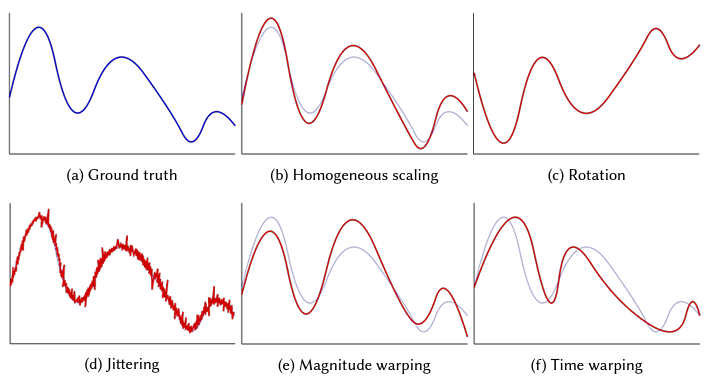
\includegraphics[width=\textwidth]{Slides/figures/Tema 3/DA_Signals.png}
    \caption{\cite{iglesias2023data}}
\end{figure}
\end{frame}

\begin{frame}{Resumen}
Existen una gran cantidad de algoritmos distintos para aumentar el número de imágenes de un dataset.

En este curso, se analizarán las siguientes:
\begin{itemize}
    \item \alert{Recorte}
    \item \alert{Volteo horizontal}
    \item \alert{Volteo vertical}
    \item \alert{Rotación}
    \item \alert{Translación}
    \item \alert{Cambios en brillo}
    \item \alert{Cambios en contraste}
    \item \alert{Cambios en matiz}
    \item \alert{Cambios en la calidad}
\end{itemize}
\end{frame}

\begin{frame}{Notebook de ejemplo, data augmentation}
El siguiente notebook contiene las implementaciones de los algoritmos de data augmentation que se estudiarán.

\begin{figure}
    \centering
    
\includegraphics[width=0.4\textwidth]{Slides/figures/GoogleColab.png}
\end{figure}
\begin{itemize}
    \centering
    \item {\Large \href{https://colab.research.google.com/drive/12G2Ijal10Fa0U_3obrwKkmuSccqIGUNq?usp=sharing}{1.3-DataAugmentation.ipynb}}
\end{itemize}
\end{frame}

\begin{frame}{Recorte}
\label{section:Recorte}
\textcolor{blue}{\href{https://keras.io/api/layers/preprocessing_layers/image_augmentation/random_crop/}{Documentación de la capa RandomCrop}}
\begin{figure}
    \centering
    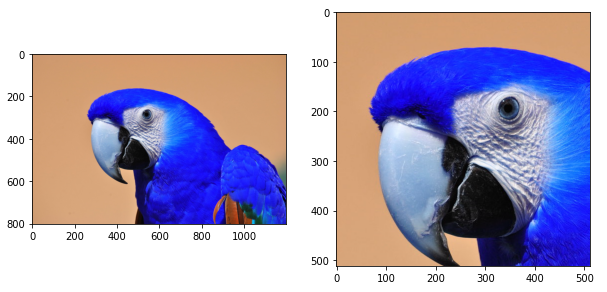
\includegraphics[width=\textwidth]{Slides/figures/Tema 3/Crop.png}
\end{figure}

* aplicar el formato \say{horizontal}
\end{frame}

\begin{frame}{Volteo horizontal}
\textcolor{blue}{\href{https://keras.io/api/layers/preprocessing_layers/image_augmentation/random_flip/}{Documentación de la capa RandomFlip}}
\begin{figure}
    \centering
    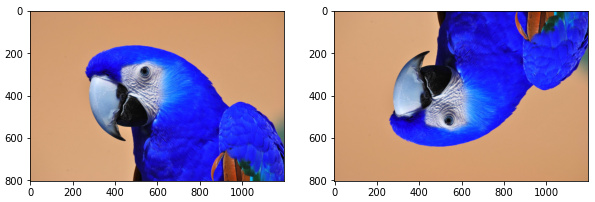
\includegraphics[width=\textwidth]{Slides/figures/Tema 3/VerFlip.png}
\end{figure}

* aplicar el formato \say{vertical}
\end{frame}

\begin{frame}{Rotación}
\textcolor{blue}{\href{https://keras.io/api/layers/preprocessing_layers/image_augmentation/random_rotation/}{Documentación de la capa RandomRotation}}
\begin{figure}
    \centering
    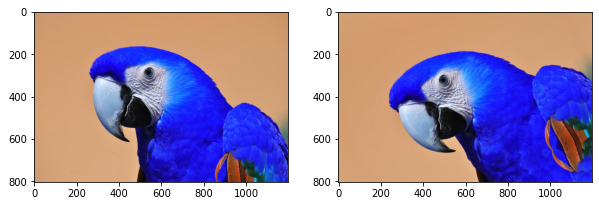
\includegraphics[width=\textwidth]{Slides/figures/Tema 3/Rotation.png}
\end{figure}
\end{frame}

\begin{frame}{Translación}
\textcolor{blue}{\href{https://keras.io/api/layers/preprocessing_layers/image_augmentation/random_translation/}{Documentación de la capa RandomTranslation}}
\begin{figure}
    \centering
    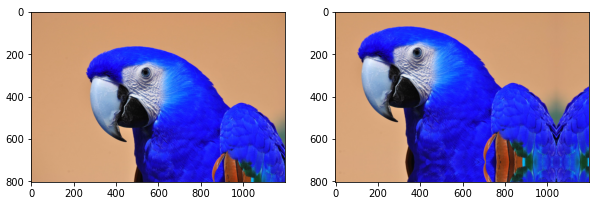
\includegraphics[width=\textwidth]{Slides/figures/Tema 3/Translation.png}
\end{figure}
\end{frame}

\begin{frame}{Cambios en contraste}
\textcolor{blue}{\href{https://keras.io/api/layers/preprocessing_layers/image_augmentation/random_contrast/}{Documentación de la capa RandomContrast}}
\begin{figure}
    \centering
    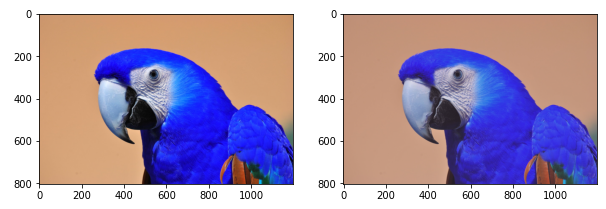
\includegraphics[width=\textwidth]{Slides/figures/Tema 3/Contrast.png}
\end{figure}
\end{frame}

\begin{frame}{Cambios en brillo}
\textcolor{blue}{\href{https://www.tensorflow.org/api_docs/python/tf/image/stateless_random_brightness}{Documentación de la capa stateless\_random\_brightness}}
\begin{figure}
    \centering
    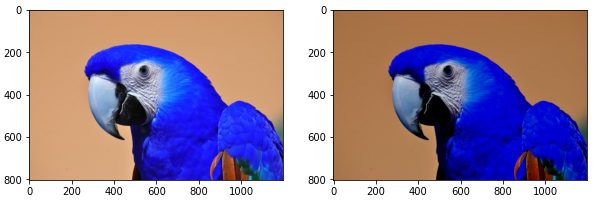
\includegraphics[width=\textwidth]{Slides/figures/Tema 3/Birghtness.png}
\end{figure}
\end{frame}

\begin{frame}{Cambios en matiz}
\textcolor{blue}{\href{https://www.tensorflow.org/api_docs/python/tf/image/stateless_random_hue}{Documentación de la capa stateless\_random\_hue}}
\begin{figure}
    \centering
    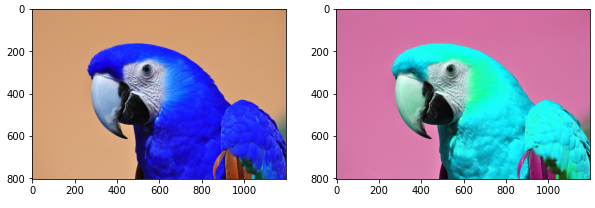
\includegraphics[width=\textwidth]{Slides/figures/Tema 3/Hue.png}
\end{figure}
\end{frame}

\begin{frame}{Cambios en calidad}
\textcolor{blue}{\href{https://www.tensorflow.org/api_docs/python/tf/image/stateless_random_jpeg_quality}{Documentación de la capa stateless\_random\_jpeg\_quality}}
\begin{figure}
    \centering
    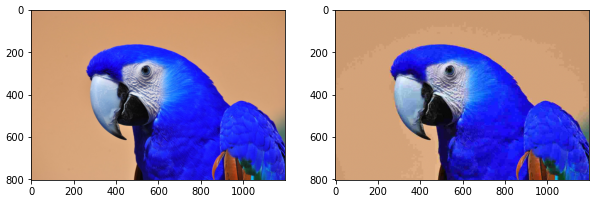
\includegraphics[width=\textwidth]{Slides/figures/Tema 3/Quality.png}
\end{figure}
\end{frame}

\begin{frame}{Implementación en Keras}
Existen dos posibilidades a la hora de realizar la implementación de los métodos de aumento de datos a la hora de realizar \alert{entrenamientos} con redes neuronales.

\begin{itemize}
    \item Capas de aumento de datos \alert{dentro del modelo}.
    \item Aumento de datos aplicado directamente al \alert{dataset}.
\end{itemize}
\end{frame}

\begin{frame}{Capas de data augmentation dentro del modelo}
A la hora de crear un modelo con las librerías \alert{Tensorflow/Keras} se pueden aplicar nuevas capas de aumento de datos en la \alert{entrada} del modelo.

Esto hará que cada vez que el modelo \alert{reciba las imágenes} como entrada, les aplique aleatoriamente las \alert{transformaciones} deseadas.

\begin{figure}
    \centering
    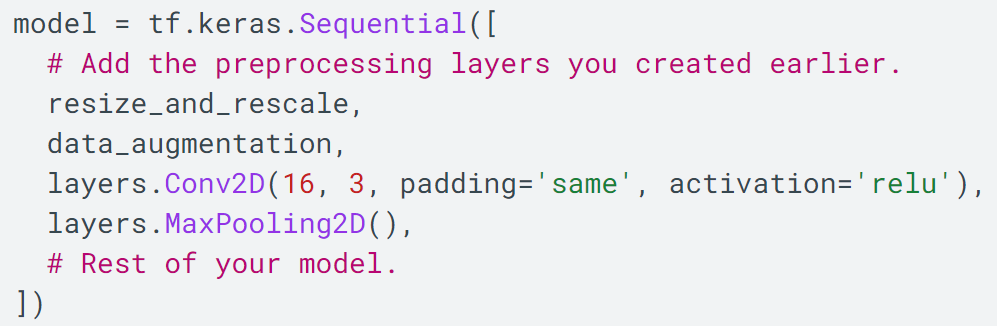
\includegraphics[width=\textwidth]{Slides/figures/Tema 3/DAKeras_1.png}
\end{figure}
\end{frame}

\begin{frame}{Data augmentation al dataset}
Otra alternativa es la de aplicar el aumento de datos \alert{después de cargar el dataset}

\begin{figure}
    \centering
    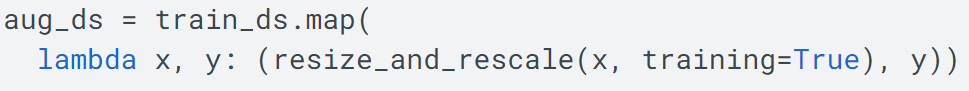
\includegraphics[width=\textwidth]{Slides/figures/Tema 3/DAKeras_2.png}
\end{figure}

\textit{* para más información se puede consultar la siguiente \textcolor{blue}{\href{https://www.tensorflow.org/tutorials/images/data_augmentation}{guía oficial de Keras}}}
\end{frame}

\addcontentsline{toc}{section}{Referencias}

\begin{frame}[allowframebreaks]{Referencias}
    \bibliographystyle{unsrt}
    \bibliography{Slides/references.bib}
\end{frame}

\begin{frame}{Contribuciones de las diapositivas}
\begin{itemize}
    \item \textbf{Autor original de las diapositivas:} Guillermo Iglesias Hernández
\end{itemize}
\end{frame}

\end{document}